\documentclass[10pt,aspectratio=169]{beamer}
\usepackage[utf8]{inputenc}
\usepackage[T1]{fontenc}
\usepackage{lmodern}
\usepackage{amsmath}
\usepackage{amsfonts}
\usepackage{amssymb}
\usepackage{graphicx}
\usepackage{hyperref}
\usepackage{listings}
\usepackage{xcolor}
\usepackage[11pt]{moresize}

\definecolor{codegreen}{rgb}{0,0.6,0}
\definecolor{codegray}{rgb}{0.5,0.5,0.5}
\definecolor{codepurple}{rgb}{0.58,0,0.82}
\definecolor{backcolour}{rgb}{0.95,0.95,0.92}

\lstdefinestyle{standard}{
	backgroundcolor=\color{backcolour},   
	commentstyle=\color{codegreen},
	keywordstyle=\color{magenta},
	numberstyle=\color{codegray},
	stringstyle=\color{codepurple},
	basicstyle=\ttfamily\tiny,
	breakatwhitespace=false,         
	breaklines=true,                 
	captionpos=b,                    
	keepspaces=true,             
	numbersep=5pt,                  
	showspaces=false,                
	showstringspaces=false,
	showtabs=false,                  
	tabsize=4
}
\lstset{style=standard}

\usetheme{Singapore}
\begin{document}
	\author{Quan Gan}
	\title{Introduction to DGL}
	%\subtitle{}
	%\logo{}
	\institute{AWS Shanghai AI Lab}
	%\date{}
	%\subject{}
	%\setbeamercovered{transparent}
	\setbeamertemplate{navigation symbols}{}
	\begin{frame}[plain]
		\maketitle
	\end{frame}
	
	\begin{frame}
		\frametitle{Recap: Graph Neural Networks}
		$$
		h^{(k)}_v = \phi\left(
		h^{(k-1)}_v,
		h^{(k)}_{\mathcal{N}(v)}
		\right) \qquad h^{(k)}_{\mathcal{N}(v)} = f\left(
		\left\lbrace
		h^{(k-1)}_u : u \in \mathcal{N}(v)
		\right\rbrace
		\right) \footnote{Xu et al., \emph{How Powerful Are Graph Neural Networks?}, ICLR 2019}
		$$
		\begin{center}
			\centering
			\only<1>{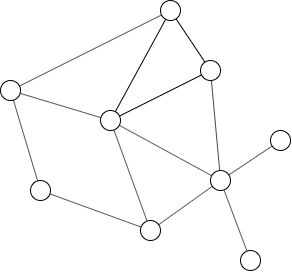
\includegraphics[width=0.4\textwidth]{graph-1.png}}
			\only<2>{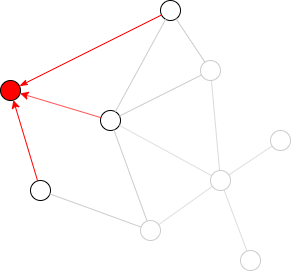
\includegraphics[width=0.4\textwidth]{graph-2.png}}
			\only<3>{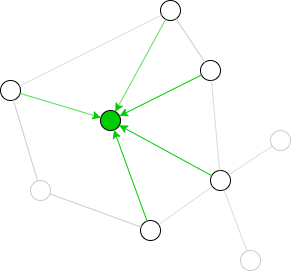
\includegraphics[width=0.4\textwidth]{graph-3.png}}
			\only<4>{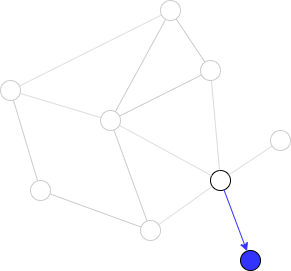
\includegraphics[width=0.4\textwidth]{graph-4.png}}
		\end{center}
	\end{frame}

	\begin{frame}[fragile]
		\frametitle{A common case\footnote{Hamilton et al., \emph{Inductive Representation Learning on Large Graphs}, NIPS 2017}}
		\begin{minipage}{0.4\textwidth}
		If $f(\cdot)$ is average:
		$$
		\begin{gathered}
		h_{\mathcal{N}(v)}^{(k)} = \dfrac{1}{\left\lvert \mathcal{N}(v) \right\rvert}
		\sum_{u \in \mathcal{N}(v)} h^{(k-1)}_u \\
		h^{(k)}_v =
		\sigma \left( W^{(k)} \left[h_v^{(k-1)} \Vert h_{\mathcal{N}(v)}^{(k)}\right] \right)
		\end{gathered}
		$$
		\end{minipage}\hfill%
		\begin{minipage}{0.5\textwidth}
			Sparse matrix multiplication, easy:
\begin{lstlisting}[language=Python]
# code: PyTorch
# src: edge source node IDs (n_nodes,)
# dst: edge destination node IDs (n_nodes,)
# H: node repr matrix (n_nodes, in_dim)
# W: weights (in_dim * 2, out_dim)
A = torch.sparse_coo_tensor(
    torch.stack([dst, src], 0),
    torch.ones(n_nodes),
    (n_nodes, n_nodes))
in_deg = torch.sparse.sum(A, 1).to_dense()
H_N = A @ H / in_deg.unsqueeze(1)
H = torch.relu(torch.cat([H_N, H], 1) @ W)
\end{lstlisting}
		\end{minipage}
	\end{frame}

	\begin{frame}[fragile]
		\frametitle{How about max pooling?}
		
		\begin{minipage}{0.4\textwidth}
			$$
			\begin{gathered}
			h_{\mathcal{N}(v)}^{(k)} =
			\max_{u \in \mathcal{N}(v)} h^{(k-1)}_u \\
			h^{(k)}_v =
			\sigma \left( W^{(k)} \left[h_v^{(k-1)} \Vert h_{\mathcal{N}(v)}^{(k)}\right] \right)
			\end{gathered}
			$$
		\end{minipage}\hfill%
		\begin{minipage}{0.5\textwidth}
			Only Tensorflow supports what we need natively:
\begin{lstlisting}[language=Python]
# code: Tensorflow 2
# src: edge source node IDs (n_nodes,)
# dst: edge destination node IDs (n_nodes,)
# H: node repr matrix (n_nodes, in_dim)
# W: weights (in_dim * 2, out_dim)

# Broadcast source features to edges
H_src = tf.gather(H, src)
H_N = tf.math.unsorted_segment_max(
    H_src, dst, n_nodes)
H = tf.nn.relu(tf.concat([H_N, H], 1) @ W)
\end{lstlisting}
		\end{minipage}
	\end{frame}

	\begin{frame}[fragile]
		\frametitle{With attention?\footnote{Velickovic et al., \emph{Graph Attention Networks}, ICLR 2018}}
		\begin{minipage}{0.4\textwidth}
			If $f(\cdot)$ is a \emph{weighted} summation:
			$$
			\begin{gathered}
			\hat\alpha ^{(k-1)}_{v,u} = MLP\left(\left[h_v^{(k-1)} \Vert h_u^{(k-1)}\right]\right) \\
			\alpha^{(k-1)}_{v,u} = softmax_j\left(
			\hat\alpha ^{(k-1)}_{v,u}
			\right)\\
			h_{\mathcal{N}(v)}^{(k)} =
			\sum_{u \in \mathcal{N}(v)} \alpha^{(k-1)}_{v,u} h^{(k-1)}_u \\
			h^{(k)}_v =
			\sigma \left( W^{(k)} \left[h_v^{(k-1)}; h_{\mathcal{N}(v)}^{(k)}\right] \right)
			\end{gathered}
			$$
		\end{minipage}\hfill%
		\begin{minipage}{0.5\textwidth}
			Can't do it easily with vanilla PyTorch/MXNet.  Possible in Tensorflow
\begin{lstlisting}[language=Python]
# code: Tensorflow 2
# src: edge source node IDs (n_nodes,)
# dst: edge destination node IDs (n_nodes,)
# H: node repr matrix (n_nodes, in_dim)
# W: weights (in_dim * 2, out_dim)
H_src = tf.gather(H, src)
H_dst = tf.gather(H, dst)
alpha_hat = MLP(tf.concat([H_dst, H_src], 1))
alpha_hat_sp = tf.sparse.SparseTensor(
    tf.stack([dst, src], 1),
    alpha_hat,
    (n_nodes, n_nodes))
alpha = tf.sparse.softmax(alpha_hat_sp)
H_N = tf.sparse.sparse_dense_matmul(alpha, H)
H = tf.nn.relu(tf.concat([H_N, H], 1) @ W)
\end{lstlisting}
		\end{minipage}
	\end{frame}

	\begin{frame}[fragile]
		\frametitle{How about LSTM\footnote{Fan et al., \emph{Metapath-guided Heterogeneous Graph Neural Network for Intent Recommendation}, KDD 2019}\footnote{Zhang et al., \emph{HetGNN: Heterogeneous Graph Neural Network}, KDD 2019}?}
		\begin{minipage}{0.4\textwidth}
			If $f(\cdot)$ is summation:
			$$
			\begin{gathered}
			h_{\mathcal{N}(v)}^{(k)} =
			LSTM( h^{(k-1)}_{u_1}, \dots, h^{(k-1)}_{u_n} ) \\
			\text{where } u_i\in \mathcal{N}(v) \text{ are in some order} \\
			h^{(k)}_v =
			\sigma \left( W^{(k)} \left[h_v^{(k-1)} \Vert h_{\mathcal{N}(v)}^{(k)}\right] \right)
			\end{gathered}
			$$
		\end{minipage}\hfill%
		\begin{minipage}{0.5\textwidth}
			Very complicated:
\begin{lstlisting}[language=Python]
# code: PyTorch
# src: edge source node IDs (n_nodes,)
# dst: edge destination node IDs (n_nodes,)
# t: timestamp of edges.
#    LSTM will go through messages in the order
#    of timestamps
# H: node repr matrix (n_nodes, in_dim)
# lstm: LSTM module
# W: weights (in_dim * 2, out_dim)
from torch.nn.utils.rnn import pack_sequence
# Build adjacency list
adjlist = []
for v in range(10): 
    v_mask = (dst == v) 
    t_v = t[v_mask] 
    N_v = src[v_mask] 
    indices = t_v.argsort() 
    adjlist.append(N_v[indices])
# Pack input sequence
seqs = [H[u] for u in adjlist]
packed_seq = pack_sequence(seqs, False)
# Run LSTM and compute the new H
_, (H_N, _) = lstm(packed_seq)
H = torch.relu(torch.cat([H_N, H], 1) @ W)
\end{lstlisting}
		\end{minipage}
	\end{frame}

	\begin{frame}
		\begin{itemize}
			\item So for each aggregation and message computation
			we have to write different code.
			\item In contrast, let's see how DGL handles the four cases.
		\end{itemize}
	\end{frame}

	\begin{frame}[fragile]
		\frametitle{A common case}
		\begin{minipage}{0.4\textwidth}
			If $f(\cdot)$ is average:
			$$
			\begin{gathered}
			h_{\mathcal{N}(v)}^{(k)} = \dfrac{1}{\left\lvert \mathcal{N}(v) \right\rvert}
			\sum_{u \in \mathcal{N}(v)} h^{(k-1)}_u \\
			h^{(k)}_v =
			\sigma \left( W^{(k)} \left[h_v^{(k-1)} \Vert h_{\mathcal{N}(v)}^{(k)}\right] \right)
			\end{gathered}
			$$
		\end{minipage}\hfill%
		\begin{minipage}{0.5\textwidth}
\begin{lstlisting}[language=Python]
# code: PyTorch
# src: edge source node IDs (n_nodes,)
# dst: edge destination node IDs (n_nodes,)
# H: node repr matrix (n_nodes, in_dim)
# W: weights (in_dim * 2, out_dim)
A = torch.sparse_coo_tensor(
    torch.stack([dst, src], 0),
    torch.ones(n_nodes),
    (n_nodes, n_nodes))
in_deg = torch.sparse.sum(A, 1).to_dense()
H_N = A @ H / in_deg.unsqueeze(1)
H = torch.relu(torch.cat([H_N, H], 1) @ W)
\end{lstlisting}

\begin{lstlisting}[language=Python]
# code: PyTorch + DGL
# G: DGL Graph
# H: node repr matrix (n_nodes, in_dim)
# W: weights (in_dim * 2, out_dim)
import dgl.function as fn
G.ndata['h'] = H
G.update_all(fn.copy_u('h', 'm'), fn.mean('m', 'h_n'))
H_N = G.ndata['h_n']
H = torch.relu(torch.cat([H_N, H], 1) @ W)
\end{lstlisting}

\begin{lstlisting}[language=Python]
# code: PyTorch + DGL
# G: DGL Graph
# H: node repr matrix (n_nodes, in_dim)
# For popular models we also have PyTorch/MXNet NN Modules:
from dgl.nn.pytorch import SAGEConv
conv = SAGEConv(in_dim * 2, out_dim, 'mean')
H = conv(G, H)
\end{lstlisting}
		\end{minipage}
	\end{frame}

	\begin{frame}[fragile]
		\frametitle{How about max pooling?}
		
		\begin{minipage}{0.4\textwidth}
			$$
			\begin{gathered}
			h_{\mathcal{N}(v)}^{(k)} =
			\max_{u \in \mathcal{N}(v)} h^{(k-1)}_u \\
			h^{(k)}_v =
			\sigma \left( W^{(k)} \left[h_v^{(k-1)} \Vert h_{\mathcal{N}(v)}^{(k)}\right] \right)
			\end{gathered}
			$$
		\end{minipage}\hfill%
		\begin{minipage}{0.5\textwidth}
\begin{lstlisting}[language=Python]
# code: Tensorflow 2
# src: edge source node IDs (n_nodes,)
# dst: edge destination node IDs (n_nodes,)
# H: node repr matrix (n_nodes, in_dim)
# W: weights (in_dim * 2, out_dim)

# Broadcast source features to edges
H_src = tf.gather(H, src)
H_N = tf.math.unsorted_segment_max(
    H_src, dst, n_nodes)
H = tf.nn.relu(tf.concat([H_N, H], 1) @ W)
\end{lstlisting}

\begin{lstlisting}[language=Python]
# code: PyTorch + DGL
# G: DGL Graph
# H: node repr matrix (n_nodes, in_dim)
# W: weights (in_dim * 2, out_dim)
import dgl.function as fn
G.ndata['h'] = H
# NOT broadcasting source features to edges
G.update_all(fn.copy_u('h', 'm'), fn.max('m', 'h_n'))
H_N = G.ndata['h_n']
H = torch.relu(torch.cat([H_N, H], 1) @ W)
\end{lstlisting}
		\end{minipage}
	\end{frame}

	\begin{frame}[fragile]
		\frametitle{With attention?}
		\begin{minipage}{0.4\textwidth}
			If $f(\cdot)$ is a \emph{weighted} summation:
			$$
			\begin{gathered}
			\hat\alpha ^{(k-1)}_{v,u} = MLP\left(\left[h_v^{(k-1)} \Vert h_u^{(k-1)}\right]\right) \\
			\alpha^{(k-1)}_{v,u} = softmax_j\left(
			\hat\alpha ^{(k-1)}_{v,u}
			\right)\\
			h_{\mathcal{N}(v)}^{(k)} =
			\sum_{u \in \mathcal{N}(v)} \alpha^{(k-1)}_{v,u} h^{(k-1)}_u \\
			h^{(k)}_v =
			\sigma \left( W^{(k)} \left[h_v^{(k-1)}; h_{\mathcal{N}(v)}^{(k)}\right] \right)
			\end{gathered}
			$$
		\end{minipage}\hfill%
		\begin{minipage}{0.5\textwidth}
			One can write his/her own message and aggregation functions:
\begin{lstlisting}[language=Python]
# code: PyTorch + DGL
# G: DGL Graph
# H: node repr matrix (n_nodes, in_dim)
# W: weights (in_dim * 2, out_dim)
def msg_func(edges):
    h_src = edges.src['h']
    h_dst = edges.dst['h']
    alpha_hat = MLP(torch.cat([h_dst, h_src], 1))
    return {'m': h_src, 'alpha_hat': alpha}

def reduce_func(nodes):
    # Incoming messages are batched along 2nd axis.
    # m has a shape of
    # (n_nodes_in_batch, in_degrees, msg_dims)
    m = nodes.mailbox['m']
    # alpha_hat has a shape of
    # (n_nodes_in_batch, in_degrees)
    alpha_hat = nodes.mailbox['alpha_hat']
    
    alpha = torch.softmax(alpha_hat, 1)
    return {'h_n': (m * alpha[:, None]).sum(1)}

import dgl.function as fn
G.ndata['h'] = H
G.update_all(msg_func, reduce_func)
H_N = G.ndata['h_n']
H = torch.relu(torch.cat([H_N, H], 1) @ W)
\end{lstlisting}
		\end{minipage}
	\end{frame}


	\begin{frame}[fragile]
	\frametitle{With attention?}
	\begin{minipage}{0.4\textwidth}
		If $f(\cdot)$ is a \emph{weighted} summation:
		$$
		\begin{gathered}
		\hat\alpha ^{(k-1)}_{v,u} = MLP\left(\left[h_v^{(k-1)} \Vert h_u^{(k-1)}\right]\right) \\
		\alpha^{(k-1)}_{v,u} = softmax_j\left(
		\hat\alpha ^{(k-1)}_{v,u}
		\right)\\
		h_{\mathcal{N}(v)}^{(k)} =
		\sum_{u \in \mathcal{N}(v)} \alpha^{(k-1)}_{v,u} h^{(k-1)}_u \\
		h^{(k)}_v =
		\sigma \left( W^{(k)} \left[h_v^{(k-1)}; h_{\mathcal{N}(v)}^{(k)}\right] \right)
		\end{gathered}
		$$
	\end{minipage}\hfill%
	\begin{minipage}{0.5\textwidth}
		Built-in message/reduce functions are more time-/memory-efficient.
\begin{lstlisting}[language=Python]
# code: PyTorch + DGL
# G: DGL Graph
# H: node repr matrix (n_nodes, in_dim)
# W: weights (in_dim * 2, out_dim)
# edge_softmax uses built-ins in computation
from dgl.nn.pytorch import edge_softmax
import dgl.function as fn
def msg(edges):
    h_src = edges.src['h']
    h_dst = edges.dst['h']
    return {'alpha': MLP(torch.cat([h_dst, h_src], 1))}

G.ndata['h'] = H
G.apply_edges(msg)  # Edges now have a feature called 'alpha'
G.edata['alpha'] = edge_softmax(G, G.edata['alpha'])
G.update_all(
    fn.u_mul_e('h', 'alpha', 'm'), fn.sum('m', 'h_n'))
H_N = G.ndata['h_n']
H = torch.relu(torch.cat([H_N, H], 1) @ W)
\end{lstlisting}
		\end{minipage}
	\end{frame}

	\begin{frame}[fragile]
		\frametitle{How about LSTM?}
		\begin{minipage}{0.4\textwidth}
			If $f(\cdot)$ is summation:
			$$
			\begin{gathered}
			h_{\mathcal{N}(v)}^{(k)} =
			LSTM( h^{(k-1)}_{u_1}, \dots, h^{(k-1)}_{u_n} ) \\
			\text{where } u_i\in \mathcal{N}(v) \text{ are in some order} \\
			h^{(k)}_v =
			\sigma \left( W^{(k)} \left[h_v^{(k-1)} \Vert h_{\mathcal{N}(v)}^{(k)}\right] \right)
			\end{gathered}
			$$
		\end{minipage}\hfill%
		\begin{minipage}{0.5\textwidth}
\begin{lstlisting}[language=Python]
# code: PyTorch + DGL
# G: DGL Graph
# t: timestamp of edges.
#    LSTM will go through messages in the order
#    of timestamps
# H: node repr matrix (n_nodes, in_dim)
# lstm: LSTM module
# W: weights (in_dim * 2, out_dim)
def reduce_func(nodes):
    indices = nodes.mailbox['t'].argsort(1)
    m = nodes.mailbox['m']
    m_ordered = m.gather(1, t[:, :, None].expand_as(m))
    return {'h_n': lstm(m)}

import dgl.function as fn
G.ndata['h'] = H
G.update_all(fn.copy_u('h', 'm'), reduce_func)
H_N = G.ndata['h_n']
H = torch.relu(torch.cat([H_N, H], 1) @ W)
\end{lstlisting}
		\end{minipage}
	\end{frame}

	\begin{frame}[fragile]
		\frametitle{How about updating partially\footnote{Trivedi et al., \emph{Know-Evolve: Deep Temporal Reasoning for Dynamic Knowledge Graphs}, ICML 2017}\footnote{Tai et al., \emph{Improved Semantic Representations From Tree-Structured Long Short-Term Memory Networks}  (TreeLSTM), ACL 2015}?}
		DGL does not confine itself in full-graph updates; one can send messages on, and receive message along, \emph{some of} the edges at a time.
		\begin{center}
			\centering
			\begin{minipage}{0.5\textwidth}
\begin{lstlisting}[language=Python]
# code: PyTorch + DGL
# An extremely simplified version of Know-Evolve, where
# messages are sent/received in the order of edge timestamps.
# H: node repr matrix (n_nodes, in_dim)
# T: numpy array of edge timestamps
def msg_func(edges):
    return {'m': MLP_msg(edges.src['h'])}
def reduce_func(nodes):
    h_old = nodes.data['h']
    h_n = nodes.mailbox['m'].sum(1)
    return {'h': MLP_reduce(torch.cat([h_old, h_n], 1))}

G.ndata['h'] = H
distinct_T = np.sort(np.unique(T))
for t in distinct_T:
    eid = np.where(T == t)
    G.send_and_recv(eid, msg_func, reduce_func)
H_output = G.ndata['h']
\end{lstlisting}
			\end{minipage}
		\end{center}
	\end{frame}

	\begin{frame}[fragile]
		\frametitle{How about heterogeneous graphs\footnote{Schlichtkrull et al., \emph{Modeling Relational Data with Graph Convolutional Networks}}?}
		\begin{itemize}
			\item DGL supports heterogeneous graphs whose nodes and edges are typed and may have type-specific features.
			\item One can perform message passing on one edge type at a time.
		\end{itemize}
		\begin{center}
			\centering
			\begin{minipage}{0.7\textwidth}
\begin{lstlisting}[language=Python]
# code: PyTorch + DGL
# xs: node features for each node type
# ws: weights for each edge type
# g: DGL heterogeneous graph
for i, ntype in enumerate(g.ntypes):
    g.nodes[ntype].data['x'] = xs[i]

# intra-type aggregation
for i, (srctype, etype, dsttype) in enumerate(g.canonical_etypes):
    g.nodes[srctype].data['h'] = g.nodes[srctype].data['x'] @ ws[etype]
    g[srctype, etype, dsttype].update_all(
        fn.copy_u('h', 'm'), fn.mean('m', 'h_%d'))

# inter-type aggregation
for ntype in g.ntypes:
    g.nodes[ntype].data['h'] = sum(
        g.nodes[ntype].data[h_name]
        for h_name in g.nodes[ntype].data.keys()
        if h_name.startswith('h_'))
\end{lstlisting}
			\end{minipage}
		\end{center}
	\end{frame}

	\begin{frame}[fragile]
		\frametitle{How about heterogeneous graphs?}
		\begin{itemize}
			\item DGL supports heterogeneous graphs whose nodes and edges are typed and may have type-specific features.
			\item One can also perform message passing on multiple edge types, further aggregating the outcome of per-edge-type aggregation with an \emph{cross-type reducer}.
		\end{itemize}
		\begin{center}
			\centering
			\begin{minipage}{0.7\textwidth}
\begin{lstlisting}[language=Python]
# code: PyTorch + DGL
# xs: node features for each node type
# ws: weights for each edge type
# g: DGL heterogeneous graph
for i, ntype in enumerate(g.ntypes):
    g.nodes[ntype].data['x'] = xs[i]

funcs = {}
for i, (srctype, etype, dsttype) in enumerate(g.canonical_etypes):
    g.nodes[srctype].data['h%d' % i] = g.nodes[srctype].data['x'] @ ws[etype]
    funcs[(srctype, etype, dsttype)] = (
        fn.copy_u('h%d' % i, 'm'), fn.mean('m', 'h'))

# message passing
g.multi_update_all(funcs, cross_reducer='sum')
\end{lstlisting}
			\end{minipage}
		\end{center}
	\end{frame}

	\begin{frame}
		\frametitle{How about scaling to larger graphs?}
		\begin{itemize}
			\item Full-graph updates become infeasible on large graphs with millions of nodes and billions of edges.
			\item We usually sample a batch of nodes at a time to compute their representations for loss computation.
			\item Furthermore, for each node, we can choose to receive messages from only a few nodes.
			\begin{center}
				\centering
				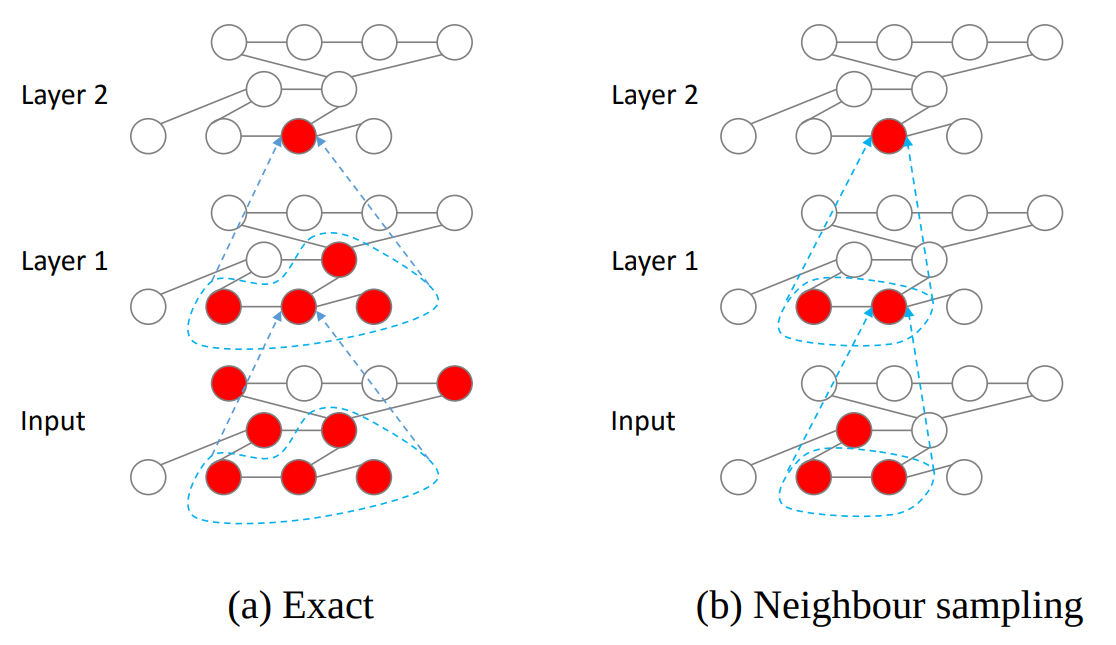
\includegraphics[width=0.5\textwidth]{nodeflow.png}
				
				\small Figure taken from Chen et al., \emph{Stochastic Training of Graph Convolutional Networks with Variance Reduction}, ICML 2018
			\end{center}
		\end{itemize}
	\end{frame}

	\begin{frame}
		\frametitle{Scaling to larger graphs (with NodeFlow)}
		For each minibatch of nodes, we explicitly construct another graph containing the dependency between nodes on each message passing layer.
		\begin{center}
			\centering
			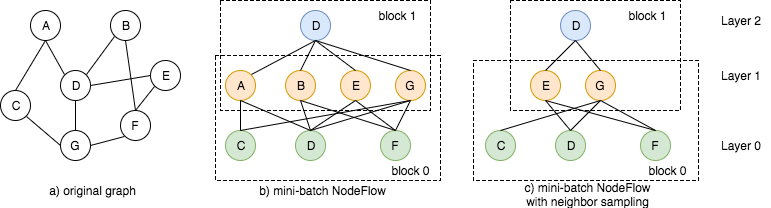
\includegraphics[width=\textwidth]{nodeflow2.png}
		\end{center}
	\end{frame}

	\begin{frame}[fragile]
		\frametitle{Scaling to larger graphs (with NodeFlow)}
		\begin{minipage}{0.45\textwidth}
\begin{lstlisting}[language=Python]
# code: MXNet + DGL
from dgl.contrib.sampling import NeighborSampler

# initialize the model and cross entropy loss
model = GCNSampling(in_feats, n_hidden, n_classes, L,
                    mx.nd.relu, dropout, prefix='GCN')
model.initialize()
loss_fcn = gluon.loss.SoftmaxCELoss()

for nf in NeighborSampler(
        g, batch_size, num_neighbors,
        neighbor_type='in', shuffle=True,
        num_hops=L, seed_nodes=train_nid):
    nf.copy_from_parent()
    with mx.autograd.record():
        # forward
        pred = model(nf)
        batch_nids = (
             nf.layer_parent_nid(-1)
             .astype('int64'))
        batch_labels = labels[batch_nids]
        # cross entropy loss
        loss = loss_fcn(pred, batch_labels)
        loss = loss.sum() / len(batch_nids)
    loss.backward()
\end{lstlisting}
		\end{minipage}\hfill%
		\begin{minipage}{0.45\textwidth}
\begin{lstlisting}[language=Python]
# code: MXNet + DGL
class GCNSampling(gluon.Block):
    # __init__ is skipped...
    
    def forward(self, nf):
        nf.layers[0].data['activation'] = \
            nf.layers[0].data['features']
        for i, MLP in enumerate(self.MLPs):
            h = nf.layers[i].data.pop('activation')
            nf.layers[i].data['h'] = h
            nf.block_compute(
                i, fn.copy_src(src='h', out='m'),
                fn.mean('m', 'h'))
            nf.layers[i + 1].data['h'] = MLP(h)
        h = nf.layers[-1].data.pop('activation')
        return h
\end{lstlisting}
		\end{minipage}
	\end{frame}

	\begin{frame}
		\frametitle{What's more?}
		\begin{itemize}
			\item Check out our repository: \url{https://github.com/dmlc/dgl}
			\begin{itemize}
				\item We have lots of PyTorch and MXNet examples!
				\item In 0.4 we also released DGL-KE, a subpackage for training knowledge graph embeddings.
			\end{itemize}
			\item Check out our documentation: \url{https://docs.dgl.ai}
			\item Discussion forum: \url{https://discuss.dgl.ai}
		\end{itemize}
	\end{frame}
\end{document}